\documentclass{beamer}

\usepackage[slovene]{babel}
\usepackage{amsfonts,amssymb}
\usepackage[utf8]{inputenc}
\usepackage{lmodern}
\usepackage[T1]{fontenc}
\usepackage{booktabs} % For better table formatting
\usepackage{xcolor}
\usepackage{tikz}

\usepackage{pgfplots}
\usepgfplotslibrary{fillbetween}
\usetikzlibrary{patterns}

\pgfplotsset{compat=1.16} 

\usetheme{Warsaw}

\def\N{\mathbb{N}} % mnozica naravnih stevil
\def\Z{\mathbb{Z}} % mnozica celih stevil
\def\Q{\mathbb{Q}} % mnozica racionalnih stevil
\def\R{\mathbb{R}} % mnozica realnih stevil
\def\C{\mathbb{C}} % mnozica kompleksnih stevil

\usepackage[margin=0.25in]{geometry}
\pgfplotsset{width=10cm,compat=1.9}
\usepgfplotslibrary{external}
\tikzexternalize

\definecolor{customGreen}{RGB}{0, 128, 0} % Darker shade of green
\definecolor{amethyst}{rgb}{0.6, 0.4, 0.8}

\def\qed{$\hfill\Box$}   % konec dokaza
\newtheorem{izrek}{Izrek}
\newtheorem{trditev}{Trditev}
\newtheorem{posledica}{Posledica}
\newtheorem{lema}{Lema}
\newtheorem{definicija}{Definicija}
\newtheorem{pripomba}{Pripomba}
\newtheorem{primer}{Primer}
\newtheorem{zgled}{Zgled}
\newtheorem{zgledi}{Zgledi uporabe}
\newtheorem{primeri_koncnih}{Primeri končnih kolobarjev}
\newtheorem{oznaka}{Oznaka}

\AtBeginEnvironment{primer}{%
  \setbeamercolor{block title}{use=example text,fg=white,bg=customGreen}
   % \setbeamercolor{block body}{parent=normal text,use=block title example,bg=block title example.bg!10!bg}
}

\AtBeginEnvironment{definicija}{%
  \setbeamercolor{block title}{use=example text,fg=white,bg=purple}
  % \setbeamercolor{block body}{parent=normal text,use=block title example,bg=block title example.bg!10!bg}
}

\AtBeginEnvironment{lema}{%
  \setbeamercolor{block title}{use=example text,fg=white,bg=amethyst}
  % \setbeamercolor{block body}{parent=normal text,use=block title example,bg=block title example.bg!10!bg}
}

\newcommand{\quot}[2]{{\raisebox{0.1em}{$#1$}\left/\raisebox{-0.2em}{$#2$}\right.}}

\title{Kratki zakoni v grupah}
\author{Jaša Knap}
\institute{Fakulteta za matematiko in fiziko \\
Oddelek za matematiko}
\date{\today}

\begin{document}


%%%%%%%%%%%%%%%%%%%%%%%%%%%%%%%%%%%%%%%%%%%%%%%%%%%%%%%%%%%%%%%%%%%%%

\begin{frame}
\titlepage
\end{frame}

%%%%%%%%%%%%%%%%%%%%%%%%%%%%%%%%%%%%%%%%%%%%%%%%%%%%%%%%%%%%%%%%%%%%%

\begin{frame}
\begin{definicija}
    \underline{Zakon v grupi $G$} je produkt abstraktnih elementov $x,y$ in njunih inverzov, ki ima lastnost, da za vsako zamenjavo $x,y$
    s konkretnima elementoma $g,h$ iz $G$ dobimo rezultat $1$ v $G$.
\end{definicija}

\begin{primer}
Grupa $G$ je Abelova natanko tedaj, ko za vsaka $x,y \in G$ velja \begin{equation*}
xy = yx \,\,\,(\iff xyx^{-1}y^{-1} = 1).
\end{equation*}  
  
\end{primer}
\end{frame}    

\begin{frame}
    \begin{primer}
    Naj bo $G$ končna grupa in $\lvert G \rvert = n$. Potem je \begin{equation*}
    x^{n} \text{ zakon.}
    \end{equation*}  
    \end{primer}

    \pause[]

    \begin{primer}
    Naj bo $G$ simetrična grupa $S_n$. Potem je \begin{equation*}
        x^{n!} \text{ zakon.}
    \end{equation*}  
    Precej krajši je zakon \begin{equation*}
        x^{\text{lcm}(1, \ldots, n)}.
    \end{equation*}  
      
    \end{primer}
    
    
\end{frame}

\begin{frame}
    \begin{itemize}
        \item \[n! \sim \sqrt{2 \pi n} \left(\frac{n}{e}\right)^n.\]
        \item \begin{equation*} 
            \text{lcm}(1,\ldots,n) \sim e^n.
        \end{equation*}  \pause[]
          
        \item Naj bo $\alpha(n)$ dolžina najkrajše besede, ki je zakon za vse grupe moči $n$ ali manj. Trenutno je znano, da je \begin{equation*}
        \alpha(n) \le  e^{155 (\log n)^4 \log(\log n)}.
        \end{equation*}  
          
    \end{itemize}
\end{frame}

\begin{frame}
    \begin{definicija}
    Naj bo $G$ grupa in naj bo $\omega$ dvočrkovna beseda. Množico \begin{equation*}
    Z(G, \omega) = \left\{ (g,h) \in  G \times  G  \middle|\, \omega(g,h) = 1 \right\} 
    \end{equation*}imenujemo \underline{izginjajoča množica besede $\omega$}.   
       
    
    \end{definicija}
    
\end{frame}

\begin{frame}
    \begin{lema}[Komutatorska lema]
    Naj bodo $\omega_1, \omega_2, \ldots, \omega_m$ dvočrkovne besede. Potem obstaja beseda $\omega$ dolžine \begin{equation*}
    l(\omega) \le  8m\left(\sum_{i=1}^{m} l\left(\omega_i\right) + m\right),
    \end{equation*}  
    za katero velja \begin{equation*}
    Z(G, \omega) \supseteq Z(G, \omega_1) \cup  Z(G, \omega_2) \cup \ldots \cup Z(G, \omega_m).
    \end{equation*}  
      
    \end{lema}
    
\end{frame}

\begin{frame}
    \begin{lema}[Razširitvena lema]
    Naj bo $G$ grupa in $N \triangleleft G$ njena edinka. Naj bo $\omega_N$ zakon za $N$ in
    $\omega_{G/N}$ zakon za kvocientno grupo $G/N$. Potem obstaja zakon $\omega$ za grupo $G$, katerega dolžina je \begin{equation*}
    l(\omega) \le  l(\omega_N)l(\omega_{G/N}).
    \end{equation*}  
      
    \end{lema}
    
% \pause[]

%     \begin{pripomba}
%     To lahko ponazorimo s kratkim eksaktnim zaporedjem: \begin{equation*}
%     1 \to N \to G \to  G / N \to 1.
%     \end{equation*}  
      
%     \end{pripomba}
    
\end{frame}

\begin{frame}
    \begin{figure}
        \centering
        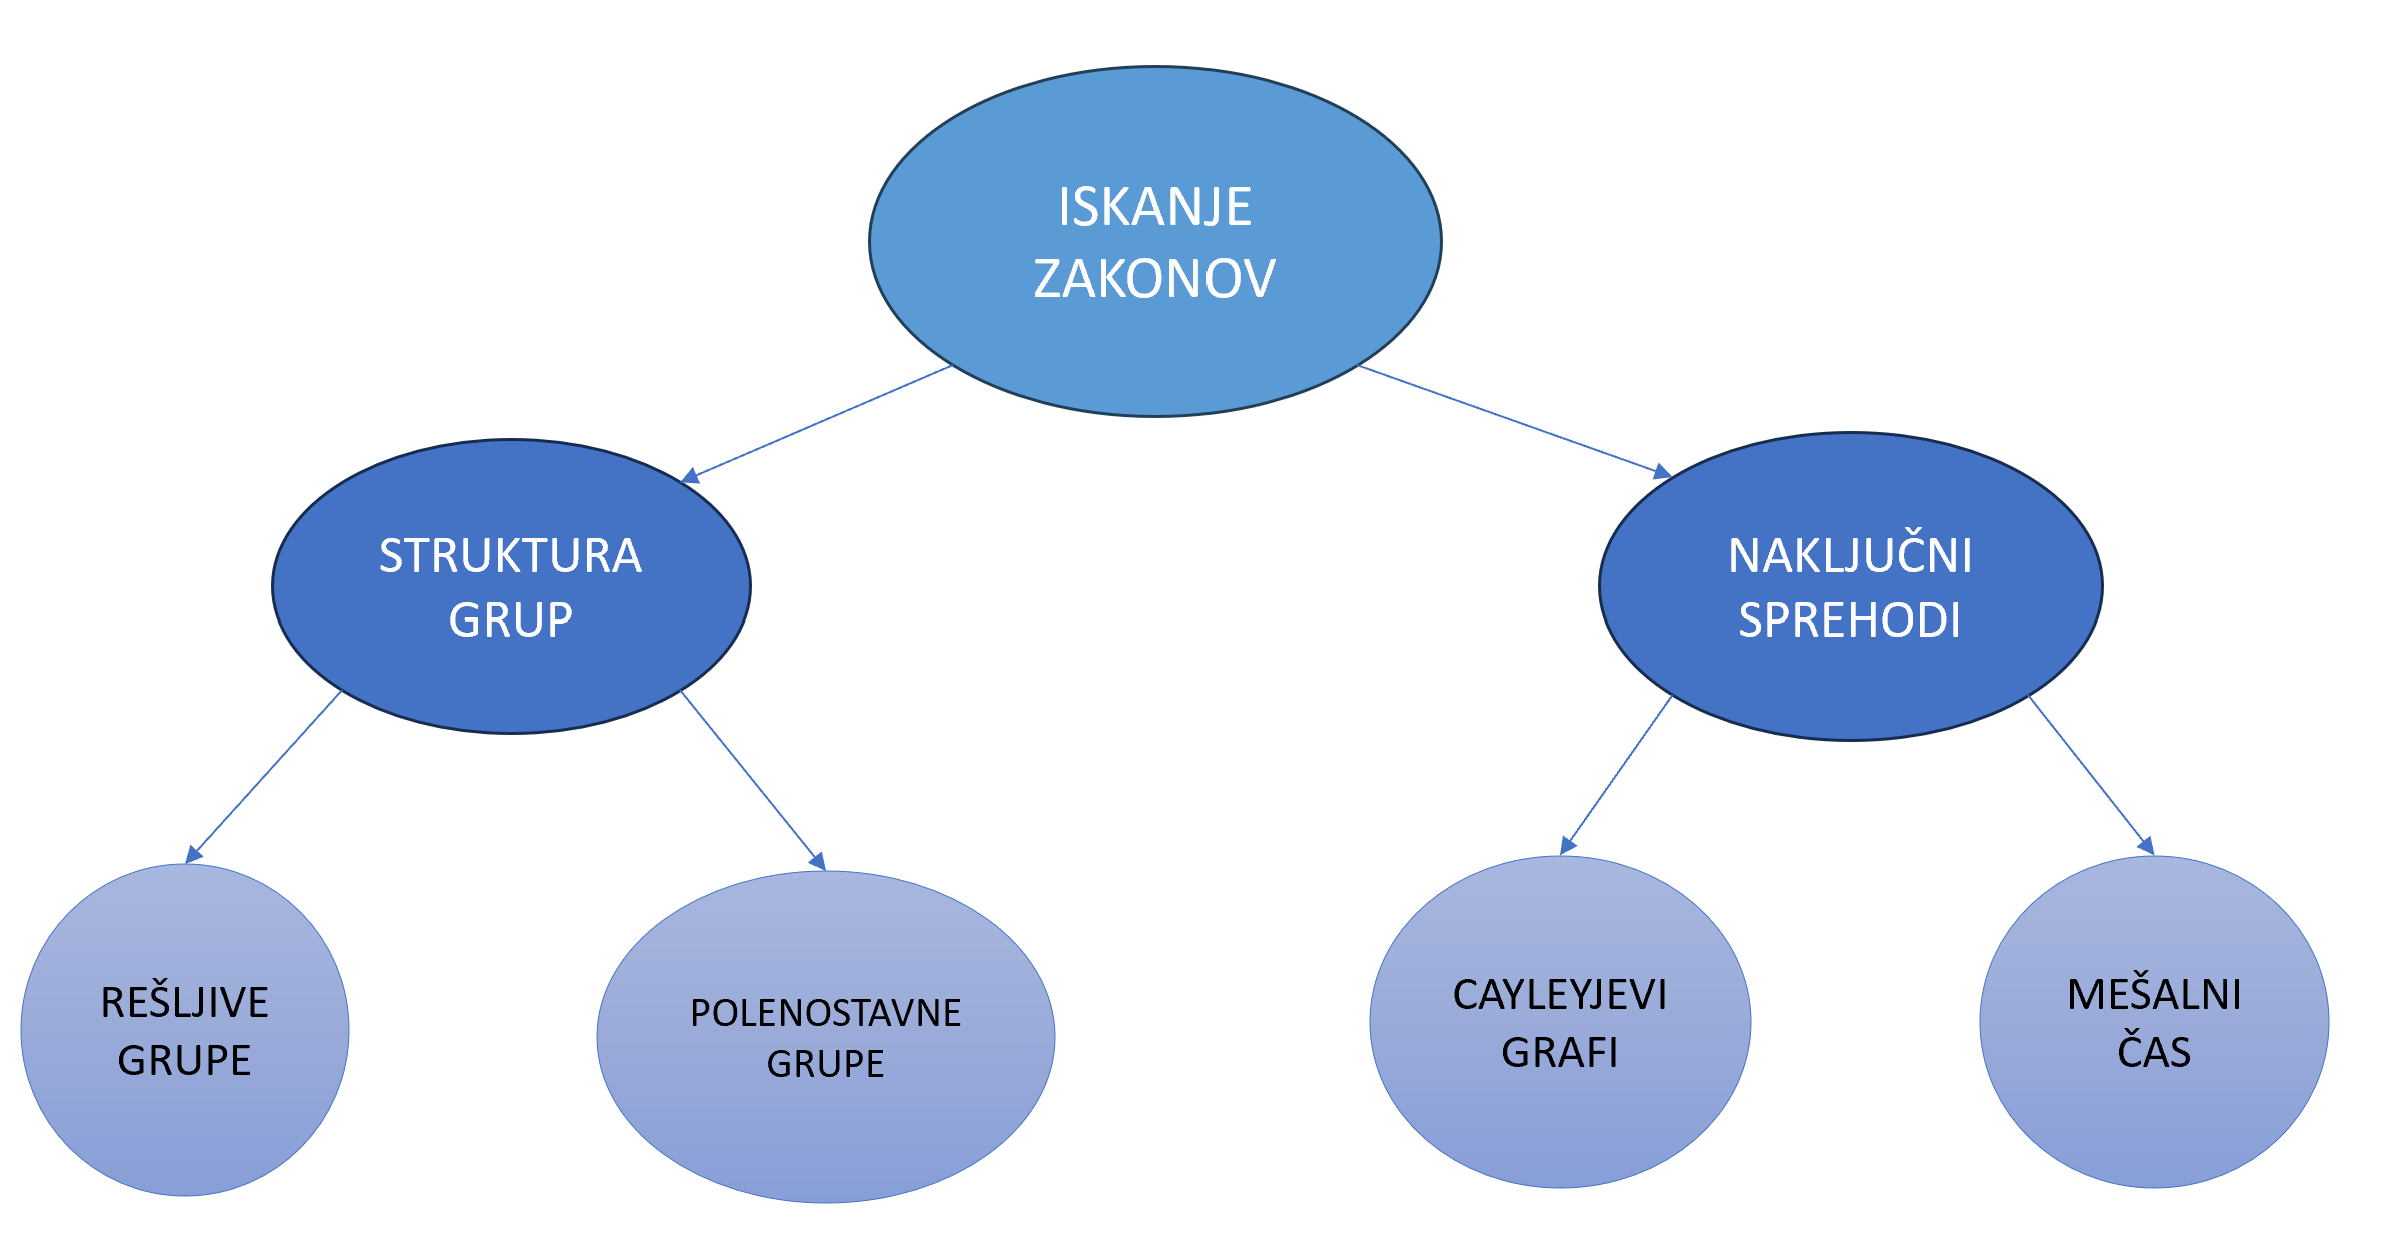
\includegraphics[width=1.05\textwidth]{Miselni vzorec.png}
        \label{fig:miselni_vzorec}
    \end{figure}
\end{frame}


\begin{frame}
Cayleyjev graf za diedrsko grupo $D_{10}$ z generatorji $\left\{ r, r^{-1}, Z \right\} $.

\begin{center}
    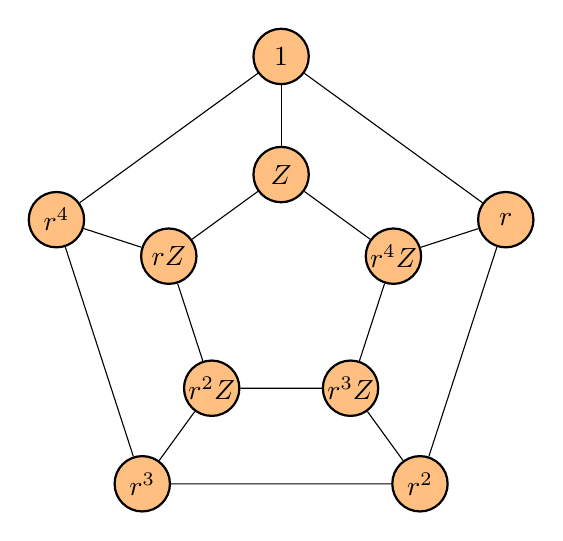
\begin{tikzpicture}[rotate=90, scale=1.5]
    \tikzset{vertex/.style={draw, thick, circle, fill=orange!50, minimum size=20pt, inner sep=0pt}}
    
    \node[vertex] (v1) at (-0*360/5:1) {$Z$};
    \node[vertex] (v2) at (-0*360/5:2) {$1$};
    \node[vertex] (v3) at (-1*360/5:1) {$r^4Z$};
    \node[vertex] (v4) at (-1*360/5:2) {$r$};
    \node[vertex] (v5) at (-2*360/5:1) {$r^3Z$};
    \node[vertex] (v6) at (-2*360/5:2) {$r^2$};
    \node[vertex] (v7) at (-3*360/5:1) {$r^2Z$};
    \node[vertex] (v8) at (-3*360/5:2) {$r^3$};
    \node[vertex] (v9) at (-4*360/5:1) {$rZ$};
    \node[vertex] (v10) at (-4*360/5:2) {$r^4$};
    
    \draw (v1) -- (v2);
    \draw (v1) -- (v3);
    \draw (v2) -- (v4);
    \draw (v3) -- (v4);
    \draw (v3) -- (v5);
    \draw (v4) -- (v6);
    \draw (v5) -- (v6);
    \draw (v5) -- (v7);
    \draw (v6) -- (v8);
    \draw (v7) -- (v8);
    \draw (v1) -- (v9);
    \draw (v7) -- (v9);
    \draw (v2) -- (v10);
    \draw (v8) -- (v10);
    \draw (v9) -- (v10);
    \end{tikzpicture}
    \end{center}
\end{frame}

% \begin{frame}
%     \begin{center}
%         Posebej zanimive so grupe $\operatorname*{PSL}_2(p^k)$ ($p$ je praštevilo, $k \in  \mathbb{N}$). 
%             % \begin{equation*}
%             %     \operatorname{PSL}_2(p^k) = \begin{cases}
%             %         \quot{\operatorname{SL}_2(p^k)}{\left\{ I \right\}} ; & p = 2  \\
%             %     \quot{\operatorname{SL}_2(p^k)}{\left\{ I, -I \right\} }; & p \neq 2
%             % \end{cases}
            
%             % \end{equation*}  
%     \end{center}

      
% \end{frame}


\end{document}

